% !TEX root =  main.tex
\section{Introduction}

AI systems have achieved impressive success with answering factual questions 
(e.g., "When was Bill Clinton born?"), using information from large-scale text or database resources~\cite{berant2013semantic,fader2014open,bordes2014open,reddy2014large,watson}. 
To scale more challenging problems that go beyond factual answer retrieval~\cite{richardson2013mctest,clark2015elementary,berantSrikumar14}, 
AI systems will need the ability to reason about the world. 
In particular they need knowledge of generalities and how it applies to the specific situations. Despite significant advances in AI, acquiring 
general knowledge and using it to reason effectively remains a huge challenge.
%and applying general knowledge about the world remains a huge challenge. 

We propose to investigate this challenge in the context of learning and reasoning about {\em processes}.
Knowledge about processes is a fundamental to part of our understanding of the world and it is 
essential to make predictions and answer questions about specific scenarios involving them.
Our goal is to develop solutions to construct a large repository of simple process knowledge 
automatically, and demonstrate its use to answer process questions that go beyond fact lookup. 

\subsection{Motivation}
We motivate the need for process knowledge using an example from an actual 4$^{th}$ grade science exam.
\begin{figure}[hbt]
	\begin{center}
	\vspace{-1em}
	% 12.08 x 1.90
	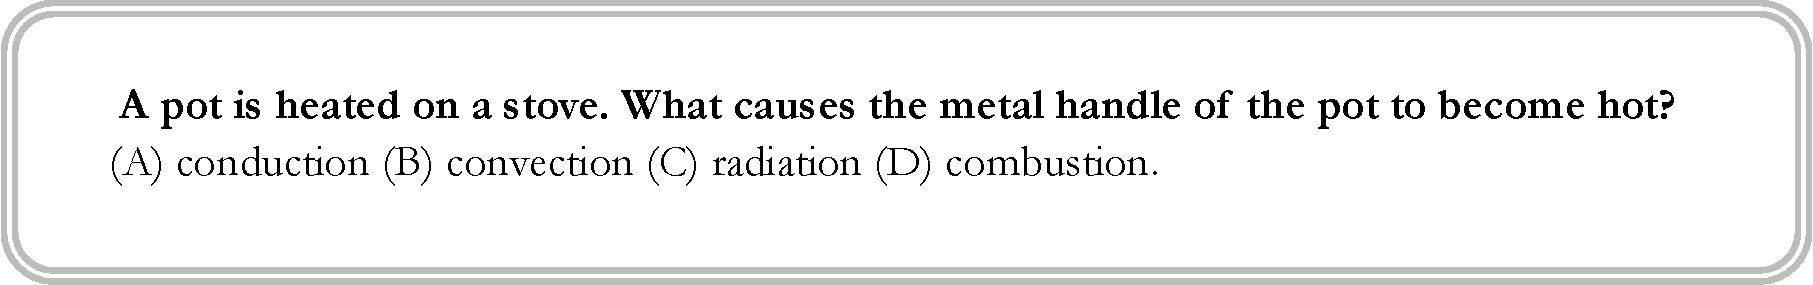
\includegraphics[width=6.04in,height=0.95in]{figures/single-question-stretch.pdf} 	
	\vspace{-1em}
	\end{center}
\end{figure}

The question tests the ability to recognize a specific scenario involving a heat transfer process.
To establish that conduction is the cause, a reasoning system must establish that there is some heat transfer happening through {\em direct contact}. 
We envision a system that first interprets the scenario and apply its knowledge about the heating process and the conduction process. 
In this case, the system needs to first identify {\em what is being heated} (the pot), and {\em what is the purported result} of the heating (the pot handle becoming hot). 
Then, knowledge about {\em heating} should allow it to conclude that the thing being heated (the pot) will become hot. 
Knowledge about {\em conduction} should suggest that anything {\em in direct contact} with a hot object (the pot handle) should also become hot.
Combining these bits the system can verify that the described scenario indeed matches the conduction process.
Replicating this type of reasoning requires knowledge about conduction and heating in a suitable computational representation.

%Specifically the knowledge about conduction should convey that there are two entities that are in direct contact, one of which is being heated or is hot, 
%and the result of conduction is that the other object also becomes {\em hot}. 

At a high level the main bits of required knowledge are: what is undergoing the process, what is the result, what is the main action etc.
These bits of information are naturally encoded as semantic roles.
PropBank~\cite{kingsbury2003propbank} and FrameNet~\cite{baker1998berkeley} are two of the highly successful efforts which provide this kind of semantic role based knowledge.
They have spurred tremendous advances in automatic semantic role labeling and their applications~\cite{gildea2002automatic,surdeanu2008conll,feizabadi2015combining,roth2015context}.
While these resources provide exhaustive coverage for modeling general open-domain actions, they only provide partial coverage on processes in the science domain.
FrameNet, for instance, does not have entries for nearly half of the processes described in 4th grade science exams. 
The coverage is likely worse for higher grade levels with deeper knowledge domains. 

In response we propose to investigate methods to automatically construct a large repository of simple knowledge about processes. Specifically, we will make three main contributions:
\begin{itemize}
\item A method for {\bf automatic extraction of process knowledge} that combines extraction and joint inference.
\item A framework for {\bf iterative knowledge expansion}, which allows the system to discover new roles
     involved in a process and expand the process representation to accommodate them.
\item The first comprehensive, large-scale {\bf knowledge base of processes}, describing the roles
      and changes involved in that process.
\end{itemize}

To provide a concrete test-bed for development and evaluation purposes, we will initially
develop this in the domain of elementary science, and evaluate it using unedited science
exam questions about processes. We expect the resource to be useful to other researchers
working in the areas of natural language processing, text processing, and question answering.

\section{Proposal Synopsis}

%\subsection{Representation}

Our primary motivation is to design a representation that effectively supports reasoning while also being amenable for automatic extraction.
We target a simple\footnote{Process knowledge is typically complex with sub-events, and temporal dependencies. They are beyond the scope of this investigation.} form of  knowledge that captures information about the entities involved and their semantic roles within the process.

We turn to the inferential needs of the target application to guide our choices.
Our preliminary work in this domain suggests a mix of {\bf pre-specified semantic roles} that apply to many processes, 
and a set of {\bf automatically induced roles} that are process specific~\cite{louvan2015:kcap}. 
We also find that we need both {\bf definitional} -- describing the key classes of entities and types of actions involved -- and {\bf instance level} knowledge about specific scenarios in which the processes occur -- providing details on the specific entities and actions. 

%process knowledge required is quite diverse, some of which is definitional in nature -- describing the key classes of entities and types of actions of a process. Others are specific to certain occurrence of the processes in specific situations or contexts -- providing details on the specific entities and actions. 
%By leveraging a common vocabulary we expect to gain from shared learning for the same roles across different processes.
%We propose to compose knowledge about each process using a set of pre-determined vocabulary of semantic roles and derive additional new roles automatically as needed.
%While many competing role sets exist, we propose a role vocabulary that covers most inferential needs in the target application~\cite{louvan2015:kcap}.

\begin{figure}[hb]
	\begin{center}
	%13.5 x 15.15
	%20.01 x 6.78
	%18.79 x 6.78
	%13.36 x 6.78
	\includegraphics[width=4.453in,height=2.26in]{figures/processkb-snippet-noqp.pdf} 	
	\caption{\label{fig:kbsnippet} 
	{An example entry for the process {\em thermal conduction}.}
	}
	\end{center}
\end{figure}

Figure~\ref{fig:kbsnippet} shows an example for the envisioned knowledge. 
The table includes a set of pre-specified general purpose roles such as {\em Undergoer}, {\em Enabler} and also a process specific role {\em Medium} that is automatically derived from inspecting sentences that describe the process. In addition to the {\em instance} role fillers, it also includes {\em definitional} type information which encodes class level information where possible.

\subsection*{Research Questions}
%Similar to FrameNet we propose to determine roles with respect to the semantics of the process rather than with respect to the specific verb (or predicate) that is used to describe the process.
%This canonicalization is desirable as it reduces reasoning time burden by eliminating need for steps that only establish equivalence of information realized via different predicates.
% %The need for a canonicalized representation precludes the direct use of existing annotations or tools built for PropBank.

There are many research challenges in automatically extracting this knowledge from text.
\begin{itemize}
\item SRL systems typically rely on large amounts of training data in order to generalize over sparse features. How can we leverage the abundance of information on the web to reduce the need for large training data?
\item A priori it is not clear how to identify which set of sentences are likely to contain relevant information.  How to gather sentences that convey the necessary knowledge? 
\item How do we account for process specific roles? 
\end{itemize}

Our investigation aims to answer these questions. 

\subsection{Automatic Extraction of Process Knowledge}
General semantic role labeling task is challenging because of the lexical and syntactic variations in role realizations. 
Handling the variations requires learning from large amounts of training data, which is laborious and requires expert labor.
%Also as discussed earlier, existing semantic resources such as FrameNet or PropBank cannot be directly used for training as they do not cover the target concepts.

Our key premise is that to gather role knowledge we don't need a semantic role labeler that works well on all sentences. 
We are interested in role acquisition and not role interpretation.
We exploit the abundance and variety of information available on the web to target extraction from 
sentences that convey the same information in expected (easy to extract) constructs and 
use joint inference to further improve performance. Our approach includes:
\begin{itemize}
\item {\bf Targeted Pattern-based Extraction} --  We build a simple pattern-based local role extractor augmented with a classifier.
Using a set of manually constructed query patterns we search the web to find sentences and extract role fillers.
A simple classifier then assesses if the extraction is valid.
%Beginning with a set of manually constructed query patterns we search the web to find sentences that match these patterns.
%For instance "<process name> causes <x>" is a simple pattern that can be used to find the {\em result} role for a process. 
Unlike traditional SRL tasks, here we have a strong expectation of the type of role and where the filler is likely to be located.
This expectation allows us to design simple structural features that generalize better across different roles and processes, 
thereby reducing need for large amounts of training data.

\item {\bf Joint Inference Across Sentences} -- We propose a joint inference model that operates over multiple sentences to avoid errors in the local extraction.
Despite the targeted acquisition, local sentence-level extraction alone is not adequate, because not all patterns are unambiguous. 
For example, "evaporates into <x>" extracts steam, a {\em result}, as well as atmosphere, a {\em location}. 
Redundancy and variety of expression on the web can help us: If the {\em atmosphere} were in fact a {\em result} then we might expect to see other sentences
where it is expressed as a result with unambiguous patterns. We propose a joint inference formulation that favors roles 
minimizing disagreements in labels for similar text spans in similar sentences.

%Because our goal is to acquire knowledge about a process, we turn the variety of expression on the web to our advantage. 
%If the {\em atmosphere} were in fact a {\em result} then we might expect to see other sentences
%where it is expressed as a result with unambiguous patterns.
%Prior work proposed Integer Linear Program (ILP) based approach for joint inference for roles {\em within} sentences.
%We build upon this work to find an assignment of roles that maximizes the sum of extraction confidences, 
%while also minimizing disagreements in labels for similar text spans in similar sentences.
\end{itemize}

\subsection{Iterative Knowledge Expansion} 
Determining the best set of knowledge bearing sentences {\em a priori} is extremely difficult. 
The quality and scope of the extracted knowledge is effectively determined by the set of sentences retrieved by the query patterns.
The query patterns may have limited coverage in some cases especially for roles that were not part of the pre-specified vocabulary.
We propose an iterative expansion of the knowledge to improve coverage of existing roles, and to discover new roles. 
An inspection of the gathered knowledge can provide valuable guidance in expanding and refining the knowledge.
We propose to investigate methods to 1) assess the coverage of the roles, 2) induce new roles by identifying consistently repeated arguments that don't fit existing roles,  
3) bootstrap extractors and query patterns using relevance feedback techniques, 4) refine the knowledge by organizing the knowledge in clusters of scenarios/instances.

\subsection{Knowledge Base of Processes}

Our target domain is grade level science. 
Based on initial analysis we estimate to generate about entries for around 2000 processes encompassing simple physical, chemical, biological, and other natural processes in this domain. 
As part of the proposed work, we propose to curate a subset of this knowledge base. Recent work has shown an effective question-based mechanism for acquiring semantic role labels
via crowd sourcing~\cite{hequestion}. To foster further research, we will release the knowledge base, and open source the code, and host web services that will allow dynamic construction of knowledge for new unseen processes. We anticipate this knowledge base will also be useful for QA in the science domain, for communities interested in AI systems, 
and to the semantic role labeling community at large.

The proposed methods will be evaluated for intrinsic quality and external utility. For internal evaluations we will perform manual evaluation of the resulting KB. 
As an external evaluation we will use the knowledge base for answering process recognition questions.

The remainder of this proposal provides details on these three main contributions.
%As part of the evaluation, {\bf we will also create a large scale curated KB, which relies on correcting the outputs from the system, rather than careful annotation of each sentence}. 
%We will also generate a gold standard of the desired roles and role fillers for evaluating coverage. As an external evaluation we will use the knowledge base for answering process recognition questions. All the %resources and evaluation test beds will be shared with the research community for further research.


\eat{\subsection{Prior Work and Contributions}

The motivation and direction for this proposal stems directly from our prior work on grade science exams.  Our earlier work studied knowledge requirements~\cite{chb2013:akbc}, developed inference-supporting rule knowledge bases~\cite{clark2014:akbc}, and investigated sophisticated state-of-the-art probabilistic reasoning methods for QA~\cite{khot2015:emlnlp}. Our ongoing preliminary work investigated the value of a handful of semantic roles in answering process recognition questions and identified the knowledge, representation, and reasoning gaps~\cite{louvan2015:kcap}. This proposal aims to address the central challenges that we've identified through these prior works.

Upon successful completion this project would have made the following contributions:
\begin{itemize}
\item {\bf Semantic Resource for Grade-level Science} -- The knowledge base we build will cover process in grade-level science and will be made available to the public and the academic community 
for fostering research in automatic reasoning systems. To foster further easy exploration, all the code will be open sourced and we will also host a web service that will dynamically compose the knowledge for new unseen processes. 
\item {\bf Targeted Acquisition and Local Extraction} -- A targeted acquisition method that gathers sentences expressing roles, and a role classification formulation that allows use of features with better generalization.
\item {\bf Joint Inference Across Sentences} -- A joint inference method that reconciles roles across different sentences.  
\item {\bf Continuous Expansion and Refinement} -- Methods for assessing expanding and refining knowledge based on the current state of the knowledge.
\end{itemize}}



